\documentclass{book}
\usepackage[a4paper,top=2.5cm,bottom=2.5cm,left=2.5cm,right=2.5cm]{geometry}
\usepackage{makeidx}
\usepackage{natbib}
\usepackage{graphicx}
\usepackage{multicol}
\usepackage{float}
\usepackage{listings}
\usepackage{color}
\usepackage{ifthen}
\usepackage[table]{xcolor}
\usepackage{textcomp}
\usepackage{alltt}
\usepackage{ifpdf}
\ifpdf
\usepackage[pdftex,
            pagebackref=true,
            colorlinks=true,
            linkcolor=blue,
            unicode
           ]{hyperref}
\else
\usepackage[ps2pdf,
            pagebackref=true,
            colorlinks=true,
            linkcolor=blue,
            unicode
           ]{hyperref}
\usepackage{pspicture}
\fi
\usepackage[utf8]{inputenc}
\usepackage{mathptmx}
\usepackage[scaled=.90]{helvet}
\usepackage{courier}
\usepackage{sectsty}
\usepackage{amssymb}
\usepackage[titles]{tocloft}
\usepackage{doxygen}
\lstset{language=C++,inputencoding=utf8,basicstyle=\footnotesize,breaklines=true,breakatwhitespace=true,tabsize=4,numbers=left }
\makeindex
\setcounter{tocdepth}{3}
\renewcommand{\footrulewidth}{0.4pt}
\renewcommand{\familydefault}{\sfdefault}
\hfuzz=15pt
\setlength{\emergencystretch}{15pt}
\hbadness=750
\tolerance=750
\begin{document}
\hypersetup{pageanchor=false,citecolor=blue}
\begin{titlepage}
\vspace*{7cm}
\begin{center}
{\Large P\-I\-M380 \\[1ex]\large 0.\-1 }\\
\vspace*{1cm}
{\large Generated by Doxygen 1.8.3.1}\\
\vspace*{0.5cm}
{\small Tue Apr 9 2013 20:29:03}\\
\end{center}
\end{titlepage}
\clearemptydoublepage
\pagenumbering{roman}
\tableofcontents
\clearemptydoublepage
\pagenumbering{arabic}
\hypersetup{pageanchor=true,citecolor=blue}
\chapter{Class Index}
\section{Class List}
Here are the classes, structs, unions and interfaces with brief descriptions\-:\begin{DoxyCompactList}
\item\contentsline{section}{\hyperlink{classBadIndex}{Bad\-Index} }{\pageref{classBadIndex}}{}
\item\contentsline{section}{\hyperlink{classCamera}{Camera} }{\pageref{classCamera}}{}
\item\contentsline{section}{\hyperlink{classColor}{Color} }{\pageref{classColor}}{}
\item\contentsline{section}{\hyperlink{classConfig}{Config} }{\pageref{classConfig}}{}
\item\contentsline{section}{\hyperlink{structCoordinate}{Coordinate} }{\pageref{structCoordinate}}{}
\item\contentsline{section}{\hyperlink{structFacePOD}{Face\-P\-O\-D} }{\pageref{structFacePOD}}{}
\item\contentsline{section}{\hyperlink{classImage}{Image} }{\pageref{classImage}}{}
\item\contentsline{section}{\hyperlink{classIncompatibleImages}{Incompatible\-Images} }{\pageref{classIncompatibleImages}}{}
\item\contentsline{section}{\hyperlink{structOtherData}{Other\-Data} }{\pageref{structOtherData}}{}
\item\contentsline{section}{\hyperlink{structOtherElem}{Other\-Elem} }{\pageref{structOtherElem}}{}
\item\contentsline{section}{\hyperlink{structPlyElement}{Ply\-Element} }{\pageref{structPlyElement}}{}
\item\contentsline{section}{\hyperlink{structPlyFile}{Ply\-File} }{\pageref{structPlyFile}}{}
\item\contentsline{section}{\hyperlink{structPlyOtherElems}{Ply\-Other\-Elems} }{\pageref{structPlyOtherElems}}{}
\item\contentsline{section}{\hyperlink{structPlyOtherProp}{Ply\-Other\-Prop} }{\pageref{structPlyOtherProp}}{}
\item\contentsline{section}{\hyperlink{structPlyProperty}{Ply\-Property} }{\pageref{structPlyProperty}}{}
\item\contentsline{section}{\hyperlink{classPointSet}{Point\-Set} }{\pageref{classPointSet}}{}
\item\contentsline{section}{\hyperlink{classVertex}{Vertex} }{\pageref{classVertex}}{}
\item\contentsline{section}{\hyperlink{structVertexPOD}{Vertex\-P\-O\-D} }{\pageref{structVertexPOD}}{}
\end{DoxyCompactList}

\chapter{Class Documentation}
\hypertarget{classBadIndex}{\section{Bad\-Index Class Reference}
\label{classBadIndex}\index{Bad\-Index@{Bad\-Index}}
}


The documentation for this class was generated from the following file\-:\begin{DoxyCompactItemize}
\item 
include/Image.\-h\end{DoxyCompactItemize}

\hypertarget{classCamera}{\section{Camera Class Reference}
\label{classCamera}\index{Camera@{Camera}}
}


Collaboration diagram for Camera\-:\nopagebreak
\begin{figure}[H]
\begin{center}
\leavevmode
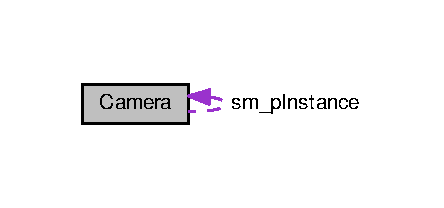
\includegraphics[width=213pt]{classCamera__coll__graph}
\end{center}
\end{figure}
\subsection*{Public Member Functions}
\begin{DoxyCompactItemize}
\item 
\hypertarget{classCamera_ae9e69218a81d66b322acea65f25557b4}{virtual Xn\-Status {\bfseries Init} (int argc, char $\ast$$\ast$argv)}\label{classCamera_ae9e69218a81d66b322acea65f25557b4}

\item 
\hypertarget{classCamera_a62c47fd66fb241f03a58d3ec6b81e9df}{virtual Xn\-Status {\bfseries Run} ()}\label{classCamera_a62c47fd66fb241f03a58d3ec6b81e9df}

\item 
\hypertarget{classCamera_a97f236804aaa6ff8c866ea7fe80e0e4b}{void {\bfseries capture\-Single\-Frame} ()}\label{classCamera_a97f236804aaa6ff8c866ea7fe80e0e4b}

\item 
\hypertarget{classCamera_afd3c41e39fdd57055223e68761384441}{std\-::string {\bfseries Int2\-Str} (int nb)}\label{classCamera_afd3c41e39fdd57055223e68761384441}

\end{DoxyCompactItemize}
\subsection*{Static Public Member Functions}
\begin{DoxyCompactItemize}
\item 
\hypertarget{classCamera_a1d0965a3b021799350ac21f14ff090f3}{static \hyperlink{classCamera}{Camera} \& {\bfseries Create\-Instance} (xn\-::\-Context \&context)}\label{classCamera_a1d0965a3b021799350ac21f14ff090f3}

\item 
\hypertarget{classCamera_afe0947fe52a6b24186f71459c4f4e1f0}{static void {\bfseries Destroy\-Instance} (\hyperlink{classCamera}{Camera} \&instance)}\label{classCamera_afe0947fe52a6b24186f71459c4f4e1f0}

\end{DoxyCompactItemize}
\subsection*{Protected Member Functions}
\begin{DoxyCompactItemize}
\item 
\hypertarget{classCamera_a745fb1420d3fac0d9fa2b4fdebdbe2ec}{{\bfseries Camera} (xn\-::\-Context \&context)}\label{classCamera_a745fb1420d3fac0d9fa2b4fdebdbe2ec}

\item 
\hypertarget{classCamera_a02c5b1e3137cf91a17c9ac1c77e1e134}{virtual int {\bfseries Display} ()}\label{classCamera_a02c5b1e3137cf91a17c9ac1c77e1e134}

\item 
\hypertarget{classCamera_a748e66e97a91728f28ee375444ab1b3c}{virtual void {\bfseries Display\-Post\-Draw} ()}\label{classCamera_a748e66e97a91728f28ee375444ab1b3c}

\item 
\hypertarget{classCamera_af81998562ee82d0815176296a4601159}{virtual void {\bfseries On\-Key} (unsigned char key, int x, int y)}\label{classCamera_af81998562ee82d0815176296a4601159}

\item 
\hypertarget{classCamera_ac98e40fcc6ff6bb43290302bf8c3e04b}{virtual Xn\-Status {\bfseries Init\-Open\-G\-L} (int argc, char $\ast$$\ast$argv)}\label{classCamera_ac98e40fcc6ff6bb43290302bf8c3e04b}

\item 
\hypertarget{classCamera_a2851c66b6f2f9a4b7526350bd9b1a7ef}{void {\bfseries Init\-Open\-G\-L\-Hooks} ()}\label{classCamera_a2851c66b6f2f9a4b7526350bd9b1a7ef}

\item 
\hypertarget{classCamera_a87d82439fc1588db3042fb2ad3c5db41}{void {\bfseries Scale\-Point} (Xn\-Point3\-D \&point)}\label{classCamera_a87d82439fc1588db3042fb2ad3c5db41}

\item 
\hypertarget{classCamera_a725592bf7b931eac09f8b102ea485cfe}{void {\bfseries gl\-Print\-String} (void $\ast$font, const char $\ast$str)}\label{classCamera_a725592bf7b931eac09f8b102ea485cfe}

\item 
\hypertarget{classCamera_a5eaafbf56e1762d806c48de70dad2901}{void {\bfseries print\-Help} (int n\-X\-Location, int $\ast$pn\-Y\-Location)}\label{classCamera_a5eaafbf56e1762d806c48de70dad2901}

\item 
\hypertarget{classCamera_a0c79141b8974f4acc4ae3a5495e24099}{void {\bfseries draw\-Help\-Screen} ()}\label{classCamera_a0c79141b8974f4acc4ae3a5495e24099}

\end{DoxyCompactItemize}
\subsection*{Static Protected Member Functions}
\begin{DoxyCompactItemize}
\item 
\hypertarget{classCamera_ac9c55b0a8dd6f567cc1b50f7196115ca}{static \hyperlink{classCamera}{Camera} \& {\bfseries Instance} ()}\label{classCamera_ac9c55b0a8dd6f567cc1b50f7196115ca}

\end{DoxyCompactItemize}
\subsection*{Protected Attributes}
\begin{DoxyCompactItemize}
\item 
\hypertarget{classCamera_a197283462b00c4fffa45696390f520f5}{xn\-::\-Context \& {\bfseries m\-\_\-r\-Context}}\label{classCamera_a197283462b00c4fffa45696390f520f5}

\item 
\hypertarget{classCamera_aae0d8e13ff6056d475eec5aa819a26c2}{xn\-::\-Depth\-Generator {\bfseries m\-\_\-depth}}\label{classCamera_aae0d8e13ff6056d475eec5aa819a26c2}

\item 
\hypertarget{classCamera_a9cd7ea9a0574f906aa9285e3629f45ac}{xn\-::\-Image\-Generator {\bfseries m\-\_\-image}}\label{classCamera_a9cd7ea9a0574f906aa9285e3629f45ac}

\item 
\hypertarget{classCamera_afe6232303a146d1da13cbf0b3ae7584c}{xn\-::\-I\-R\-Generator {\bfseries m\-\_\-\-I\-R}}\label{classCamera_afe6232303a146d1da13cbf0b3ae7584c}

\end{DoxyCompactItemize}
\subsection*{Static Protected Attributes}
\begin{DoxyCompactItemize}
\item 
\hypertarget{classCamera_a696c4f46f01f34f959e15de32d1a9c72}{static \hyperlink{classCamera}{Camera} $\ast$ {\bfseries sm\-\_\-p\-Instance} = N\-U\-L\-L}\label{classCamera_a696c4f46f01f34f959e15de32d1a9c72}

\end{DoxyCompactItemize}


The documentation for this class was generated from the following files\-:\begin{DoxyCompactItemize}
\item 
include/Camera.\-h\item 
src/Camera.\-cpp\end{DoxyCompactItemize}

\hypertarget{classColor}{\section{Color Class Reference}
\label{classColor}\index{Color@{Color}}
}
\subsection*{Public Member Functions}
\begin{DoxyCompactItemize}
\item 
\hypertarget{classColor_a8ab00b210e073f5927b81a94c7a07324}{{\bfseries Color} (const \hyperlink{classColor}{Color} \&i\-Other)}\label{classColor_a8ab00b210e073f5927b81a94c7a07324}

\item 
\hypertarget{classColor_a7e515720045da20ab9f16c5d0e0487e3}{{\bfseries Color} (int red, int green, int blue, int alpha=255)}\label{classColor_a7e515720045da20ab9f16c5d0e0487e3}

\item 
\hypertarget{classColor_ab47de2c4626ee3db857d8c19014adc0d}{{\bfseries Color} (const float red, const float green, const float blue, const float alpha=1.\-0f)}\label{classColor_ab47de2c4626ee3db857d8c19014adc0d}

\item 
\hypertarget{classColor_a5a82d6c9cc297a2f677436f644397a6c}{\hyperlink{classColor}{Color} \& {\bfseries operator=} (const \hyperlink{classColor}{Color} \&i\-Other)}\label{classColor_a5a82d6c9cc297a2f677436f644397a6c}

\end{DoxyCompactItemize}


The documentation for this class was generated from the following files\-:\begin{DoxyCompactItemize}
\item 
include/Color.\-h\item 
src/Color.\-cpp\end{DoxyCompactItemize}

\hypertarget{classConfig}{\section{Config Class Reference}
\label{classConfig}\index{Config@{Config}}
}
\subsection*{Static Public Member Functions}
\begin{DoxyCompactItemize}
\item 
\hypertarget{classConfig_a568c93f4eed136d38e6feee300a28b5d}{static void {\bfseries Load\-Configs} (const std\-::string \&i\-Filename)}\label{classConfig_a568c93f4eed136d38e6feee300a28b5d}

\item 
\hypertarget{classConfig_a3cefb1704bfbd41aa205265f218da0a0}{static const std\-::string \& {\bfseries Root\-Path} ()}\label{classConfig_a3cefb1704bfbd41aa205265f218da0a0}

\item 
\hypertarget{classConfig_a607783622e38763472830639f04a17fd}{static const std\-::string \& {\bfseries Resources\-Path} ()}\label{classConfig_a607783622e38763472830639f04a17fd}

\item 
\hypertarget{classConfig_ac3a7c38f6d1196a75b7d42d870131cec}{static const std\-::string \& {\bfseries Data\-Path} ()}\label{classConfig_ac3a7c38f6d1196a75b7d42d870131cec}

\item 
\hypertarget{classConfig_ae85d5337c5a2612a3890629ee5443e2e}{static const std\-::string \& {\bfseries Output\-Path} ()}\label{classConfig_ae85d5337c5a2612a3890629ee5443e2e}

\item 
\hypertarget{classConfig_af873ea8c47d328921d9a20b884700e76}{static const std\-::string \& {\bfseries Config\-Path} ()}\label{classConfig_af873ea8c47d328921d9a20b884700e76}

\end{DoxyCompactItemize}


The documentation for this class was generated from the following file\-:\begin{DoxyCompactItemize}
\item 
src/main.\-cpp\end{DoxyCompactItemize}

\hypertarget{structCoordinate}{\section{Coordinate Struct Reference}
\label{structCoordinate}\index{Coordinate@{Coordinate}}
}
\subsection*{Public Member Functions}
\begin{DoxyCompactItemize}
\item 
\hypertarget{structCoordinate_a7df547dd94d79a46e88d0fb57c2c9e74}{{\bfseries Coordinate} (const int \&x, const int \&y)}\label{structCoordinate_a7df547dd94d79a46e88d0fb57c2c9e74}

\end{DoxyCompactItemize}
\subsection*{Public Attributes}
\begin{DoxyCompactItemize}
\item 
\hypertarget{structCoordinate_ad462d671f1feb865911333e3ff5f0a5d}{int {\bfseries x}}\label{structCoordinate_ad462d671f1feb865911333e3ff5f0a5d}

\item 
\hypertarget{structCoordinate_a5c7d59f0f65ff9371b6c3791f78880aa}{int {\bfseries y}}\label{structCoordinate_a5c7d59f0f65ff9371b6c3791f78880aa}

\end{DoxyCompactItemize}


The documentation for this struct was generated from the following file\-:\begin{DoxyCompactItemize}
\item 
include/Image.\-h\end{DoxyCompactItemize}

\hypertarget{structFacePOD}{\section{Face\-P\-O\-D Struct Reference}
\label{structFacePOD}\index{Face\-P\-O\-D@{Face\-P\-O\-D}}
}
\subsection*{Public Attributes}
\begin{DoxyCompactItemize}
\item 
\hypertarget{structFacePOD_a546069b25daedbfd6de63e0280514026}{unsigned char {\bfseries n\-Verts}}\label{structFacePOD_a546069b25daedbfd6de63e0280514026}

\item 
\hypertarget{structFacePOD_a878bc3da31fb37c0a2eeaa03bf98db53}{int $\ast$ {\bfseries verts}}\label{structFacePOD_a878bc3da31fb37c0a2eeaa03bf98db53}

\end{DoxyCompactItemize}


The documentation for this struct was generated from the following file\-:\begin{DoxyCompactItemize}
\item 
src/Point\-Set.\-cpp\end{DoxyCompactItemize}

\hypertarget{classImage}{\section{Image Class Reference}
\label{classImage}\index{Image@{Image}}
}
\subsection*{Public Member Functions}
\begin{DoxyCompactItemize}
\item 
\hypertarget{classImage_a0f45033c76471420cb42775c91290eb8}{{\bfseries Image} (const int i\-Width, const int i\-Height, const int i\-Grey\-Level)}\label{classImage_a0f45033c76471420cb42775c91290eb8}

\item 
\hypertarget{classImage_ac2b9ea78dbf56127b04e6c2a3fdbec5f}{{\bfseries Image} (const std\-::string \&i\-Filename)}\label{classImage_ac2b9ea78dbf56127b04e6c2a3fdbec5f}

\item 
\hypertarget{classImage_a74f502d0c938bf043b91b8a4e6841a4e}{void {\bfseries Set\-Height} (const int i\-Height)}\label{classImage_a74f502d0c938bf043b91b8a4e6841a4e}

\item 
\hypertarget{classImage_ae6db09b55cca7e411ce6f474dce2b068}{void {\bfseries Set\-Width} (const int i\-Width)}\label{classImage_ae6db09b55cca7e411ce6f474dce2b068}

\item 
\hypertarget{classImage_af18b61d109c00cb7b5fc300ce5687547}{void {\bfseries Set\-Grey\-Level} (const int i\-Grey\-Level)}\label{classImage_af18b61d109c00cb7b5fc300ce5687547}

\item 
\hypertarget{classImage_a9157cb283f6b863c47f437d84dde75b3}{int const \& {\bfseries Get\-Height} () const }\label{classImage_a9157cb283f6b863c47f437d84dde75b3}

\item 
\hypertarget{classImage_a43bbe5663dc2a2550f28051aec632ec8}{int const \& {\bfseries Get\-Width} () const }\label{classImage_a43bbe5663dc2a2550f28051aec632ec8}

\item 
\hypertarget{classImage_ae2730b30cd0edc6cb90646795d3f5ff6}{int const \& {\bfseries Get\-Max\-Grey\-Level} () const }\label{classImage_ae2730b30cd0edc6cb90646795d3f5ff6}

\item 
\hypertarget{classImage_a12c9a42ef545c51051b948400005e474}{void {\bfseries Load\-From\-File} (const std\-::string \&i\-Filename)}\label{classImage_a12c9a42ef545c51051b948400005e474}

\item 
\hypertarget{classImage_a1351003ce96c6ec81f8e4b0e13e35233}{void {\bfseries Create\-Ascii\-Pgm} (const std\-::string \&i\-Filename)}\label{classImage_a1351003ce96c6ec81f8e4b0e13e35233}

\item 
\hypertarget{classImage_a30c7f00bb4c397a30e158f2da7465426}{void {\bfseries Recalculate} ()}\label{classImage_a30c7f00bb4c397a30e158f2da7465426}

\item 
\hypertarget{classImage_ad26d6cbaf59c26f9475e2b33188f398e}{float \& {\bfseries operator()} (const int i\-Row, const int i\-Col)}\label{classImage_ad26d6cbaf59c26f9475e2b33188f398e}

\item 
\hypertarget{classImage_a5fa8be39a79f9f98300e3fea8a902c59}{float {\bfseries operator()} (const int i\-Row, const int i\-Col) const }\label{classImage_a5fa8be39a79f9f98300e3fea8a902c59}

\item 
\hypertarget{classImage_a1f640b89c8f8f9d9abc69c3ccb9afaf8}{\hyperlink{classImage}{Image} {\bfseries Pattern\-Search} (const \hyperlink{classImage}{Image} \&i\-Mask, \hyperlink{structCoordinate}{Coordinate} \&o\-Best\-Match) const }\label{classImage_a1f640b89c8f8f9d9abc69c3ccb9afaf8}

\item 
\hypertarget{classImage_ae1561a04dad8a6aad0cb38933184ca02}{int {\bfseries Correlation} (const \hyperlink{classImage}{Image} \&i\-Other) const }\label{classImage_ae1561a04dad8a6aad0cb38933184ca02}

\item 
\hypertarget{classImage_a1c21f181bede39438721517ce2e64605}{\hyperlink{classImage}{Image} {\bfseries Difference} (const \hyperlink{classImage}{Image} \&i\-Other) const }\label{classImage_a1c21f181bede39438721517ce2e64605}

\end{DoxyCompactItemize}


The documentation for this class was generated from the following files\-:\begin{DoxyCompactItemize}
\item 
include/Image.\-h\item 
src/Image.\-cpp\end{DoxyCompactItemize}

\hypertarget{classIncompatibleImages}{\section{Incompatible\-Images Class Reference}
\label{classIncompatibleImages}\index{Incompatible\-Images@{Incompatible\-Images}}
}


The documentation for this class was generated from the following file\-:\begin{DoxyCompactItemize}
\item 
include/Image.\-h\end{DoxyCompactItemize}

\hypertarget{structOtherData}{\section{Other\-Data Struct Reference}
\label{structOtherData}\index{Other\-Data@{Other\-Data}}
}
\subsection*{Public Attributes}
\begin{DoxyCompactItemize}
\item 
\hypertarget{structOtherData_a21c6a90664f23db87f2e8a91c87b1ac1}{void $\ast$ {\bfseries other\-\_\-props}}\label{structOtherData_a21c6a90664f23db87f2e8a91c87b1ac1}

\end{DoxyCompactItemize}


The documentation for this struct was generated from the following file\-:\begin{DoxyCompactItemize}
\item 
include/Ply\-File.\-h\end{DoxyCompactItemize}

\hypertarget{structOtherElem}{\section{Other\-Elem Struct Reference}
\label{structOtherElem}\index{Other\-Elem@{Other\-Elem}}
}


Collaboration diagram for Other\-Elem\-:\nopagebreak
\begin{figure}[H]
\begin{center}
\leavevmode
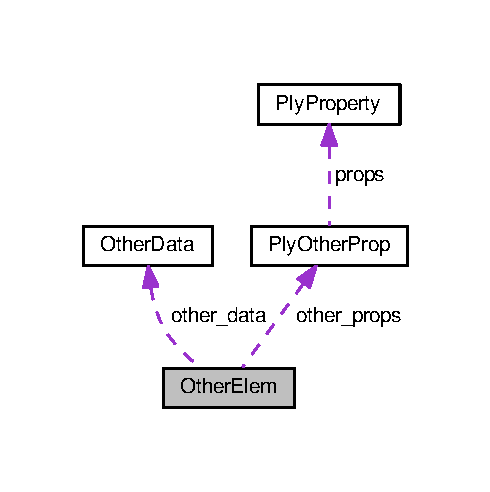
\includegraphics[width=235pt]{structOtherElem__coll__graph}
\end{center}
\end{figure}
\subsection*{Public Attributes}
\begin{DoxyCompactItemize}
\item 
\hypertarget{structOtherElem_a86011b3e2b292c7354ff8d39ab6e38f4}{char $\ast$ {\bfseries elem\-\_\-name}}\label{structOtherElem_a86011b3e2b292c7354ff8d39ab6e38f4}

\item 
\hypertarget{structOtherElem_ae94cc7f40247728d5d98971685ff35e3}{int {\bfseries elem\-\_\-count}}\label{structOtherElem_ae94cc7f40247728d5d98971685ff35e3}

\item 
\hypertarget{structOtherElem_a3dec65c2ba1b4c206ac9f3d02ec4b935}{\hyperlink{structOtherData}{Other\-Data} $\ast$$\ast$ {\bfseries other\-\_\-data}}\label{structOtherElem_a3dec65c2ba1b4c206ac9f3d02ec4b935}

\item 
\hypertarget{structOtherElem_aa800ba93c6711ef9da7be0d3cf032263}{\hyperlink{structPlyOtherProp}{Ply\-Other\-Prop} $\ast$ {\bfseries other\-\_\-props}}\label{structOtherElem_aa800ba93c6711ef9da7be0d3cf032263}

\end{DoxyCompactItemize}


The documentation for this struct was generated from the following file\-:\begin{DoxyCompactItemize}
\item 
include/Ply\-File.\-h\end{DoxyCompactItemize}

\hypertarget{structPlyElement}{\section{Ply\-Element Struct Reference}
\label{structPlyElement}\index{Ply\-Element@{Ply\-Element}}
}


Collaboration diagram for Ply\-Element\-:\nopagebreak
\begin{figure}[H]
\begin{center}
\leavevmode
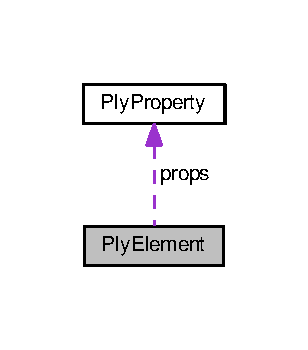
\includegraphics[width=148pt]{structPlyElement__coll__graph}
\end{center}
\end{figure}
\subsection*{Public Attributes}
\begin{DoxyCompactItemize}
\item 
\hypertarget{structPlyElement_a851bfdee0489e67d5105d7f947dc7e35}{char $\ast$ {\bfseries name}}\label{structPlyElement_a851bfdee0489e67d5105d7f947dc7e35}

\item 
\hypertarget{structPlyElement_a3975c8d9bdd3b4435bca2cb6f7e99733}{int {\bfseries num}}\label{structPlyElement_a3975c8d9bdd3b4435bca2cb6f7e99733}

\item 
\hypertarget{structPlyElement_ab4a94646827e6b91a9778a4fea45a051}{int {\bfseries size}}\label{structPlyElement_ab4a94646827e6b91a9778a4fea45a051}

\item 
\hypertarget{structPlyElement_af8251c4b09b4292a0529a7c7acfe7771}{int {\bfseries nprops}}\label{structPlyElement_af8251c4b09b4292a0529a7c7acfe7771}

\item 
\hypertarget{structPlyElement_abd25d464578a898680daea44e24fbb21}{\hyperlink{structPlyProperty}{Ply\-Property} $\ast$$\ast$ {\bfseries props}}\label{structPlyElement_abd25d464578a898680daea44e24fbb21}

\item 
\hypertarget{structPlyElement_aa0e220908f47f0c2c3a5bcee0ee01d99}{char $\ast$ {\bfseries store\-\_\-prop}}\label{structPlyElement_aa0e220908f47f0c2c3a5bcee0ee01d99}

\item 
\hypertarget{structPlyElement_a3711e7f51c082da6639ac3239ee2444a}{int {\bfseries other\-\_\-offset}}\label{structPlyElement_a3711e7f51c082da6639ac3239ee2444a}

\item 
\hypertarget{structPlyElement_a4ec699438f485c7ecca7cb7d623e4e74}{int {\bfseries other\-\_\-size}}\label{structPlyElement_a4ec699438f485c7ecca7cb7d623e4e74}

\end{DoxyCompactItemize}


The documentation for this struct was generated from the following file\-:\begin{DoxyCompactItemize}
\item 
include/Ply\-File.\-h\end{DoxyCompactItemize}

\hypertarget{structPlyFile}{\section{Ply\-File Struct Reference}
\label{structPlyFile}\index{Ply\-File@{Ply\-File}}
}


Collaboration diagram for Ply\-File\-:\nopagebreak
\begin{figure}[H]
\begin{center}
\leavevmode
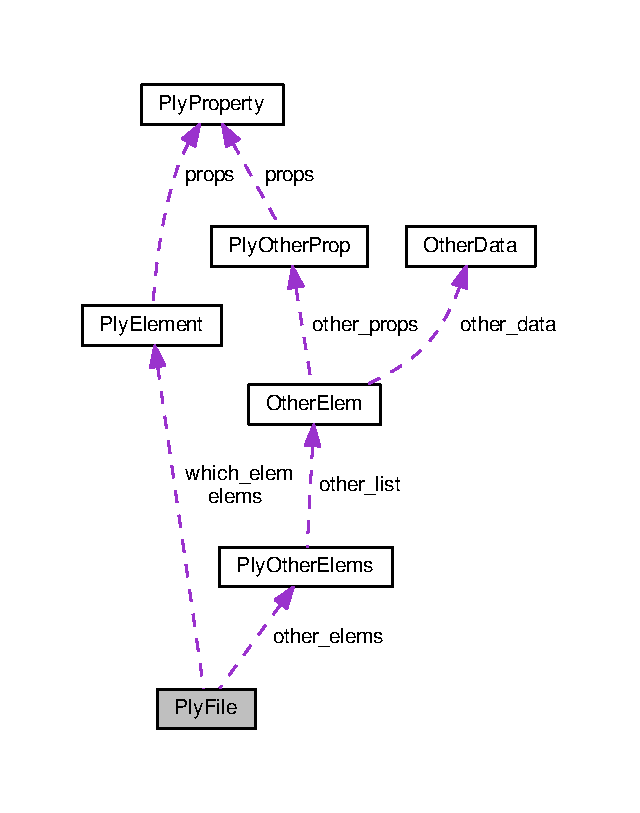
\includegraphics[width=307pt]{structPlyFile__coll__graph}
\end{center}
\end{figure}
\subsection*{Public Attributes}
\begin{DoxyCompactItemize}
\item 
\hypertarget{structPlyFile_affa03cb65d7afdc1b54ba1930da1e0ce}{F\-I\-L\-E $\ast$ {\bfseries fp}}\label{structPlyFile_affa03cb65d7afdc1b54ba1930da1e0ce}

\item 
\hypertarget{structPlyFile_ac8f47215e1cab6332c4a91735faceac1}{int {\bfseries file\-\_\-type}}\label{structPlyFile_ac8f47215e1cab6332c4a91735faceac1}

\item 
\hypertarget{structPlyFile_a54079430fc47c9303c194ecffaf9392d}{float {\bfseries version}}\label{structPlyFile_a54079430fc47c9303c194ecffaf9392d}

\item 
\hypertarget{structPlyFile_a2d94dc0c534e364b232d1ea41d64c1f1}{int {\bfseries nelems}}\label{structPlyFile_a2d94dc0c534e364b232d1ea41d64c1f1}

\item 
\hypertarget{structPlyFile_aa123ddfd8c89539dde7644d121082432}{\hyperlink{structPlyElement}{Ply\-Element} $\ast$$\ast$ {\bfseries elems}}\label{structPlyFile_aa123ddfd8c89539dde7644d121082432}

\item 
\hypertarget{structPlyFile_a033842a20f0620979d992898f6a52a14}{int {\bfseries num\-\_\-comments}}\label{structPlyFile_a033842a20f0620979d992898f6a52a14}

\item 
\hypertarget{structPlyFile_afe9f3f406d4ae2ae20d9ed0bfb9a990f}{char $\ast$$\ast$ {\bfseries comments}}\label{structPlyFile_afe9f3f406d4ae2ae20d9ed0bfb9a990f}

\item 
\hypertarget{structPlyFile_aa1a8dc64805585240d50df3192854d18}{int {\bfseries num\-\_\-obj\-\_\-info}}\label{structPlyFile_aa1a8dc64805585240d50df3192854d18}

\item 
\hypertarget{structPlyFile_a5537a09cf69258341126d00e39e13343}{char $\ast$$\ast$ {\bfseries obj\-\_\-info}}\label{structPlyFile_a5537a09cf69258341126d00e39e13343}

\item 
\hypertarget{structPlyFile_a8446d1253e51c33fc1149d87d60d91c9}{\hyperlink{structPlyElement}{Ply\-Element} $\ast$ {\bfseries which\-\_\-elem}}\label{structPlyFile_a8446d1253e51c33fc1149d87d60d91c9}

\item 
\hypertarget{structPlyFile_aceb5a35f93d4ab5df12713e1b62e838b}{\hyperlink{structPlyOtherElems}{Ply\-Other\-Elems} $\ast$ {\bfseries other\-\_\-elems}}\label{structPlyFile_aceb5a35f93d4ab5df12713e1b62e838b}

\end{DoxyCompactItemize}


The documentation for this struct was generated from the following file\-:\begin{DoxyCompactItemize}
\item 
include/Ply\-File.\-h\end{DoxyCompactItemize}

\hypertarget{structPlyOtherElems}{\section{Ply\-Other\-Elems Struct Reference}
\label{structPlyOtherElems}\index{Ply\-Other\-Elems@{Ply\-Other\-Elems}}
}


Collaboration diagram for Ply\-Other\-Elems\-:\nopagebreak
\begin{figure}[H]
\begin{center}
\leavevmode
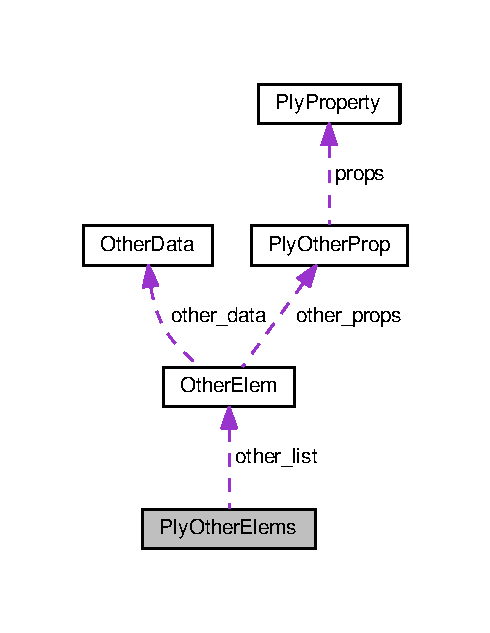
\includegraphics[width=235pt]{structPlyOtherElems__coll__graph}
\end{center}
\end{figure}
\subsection*{Public Attributes}
\begin{DoxyCompactItemize}
\item 
\hypertarget{structPlyOtherElems_ab464cc630ef0f33b64474ddf9dd00d63}{int {\bfseries num\-\_\-elems}}\label{structPlyOtherElems_ab464cc630ef0f33b64474ddf9dd00d63}

\item 
\hypertarget{structPlyOtherElems_a2a3390c0b6de21756b10ae550c66de8a}{\hyperlink{structOtherElem}{Other\-Elem} $\ast$ {\bfseries other\-\_\-list}}\label{structPlyOtherElems_a2a3390c0b6de21756b10ae550c66de8a}

\end{DoxyCompactItemize}


The documentation for this struct was generated from the following file\-:\begin{DoxyCompactItemize}
\item 
include/Ply\-File.\-h\end{DoxyCompactItemize}

\hypertarget{structPlyOtherProp}{\section{Ply\-Other\-Prop Struct Reference}
\label{structPlyOtherProp}\index{Ply\-Other\-Prop@{Ply\-Other\-Prop}}
}


Collaboration diagram for Ply\-Other\-Prop\-:\nopagebreak
\begin{figure}[H]
\begin{center}
\leavevmode
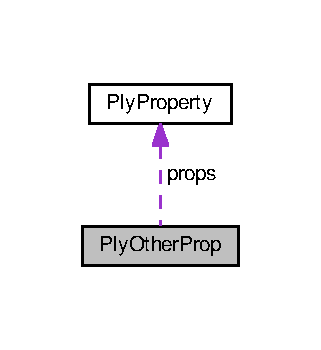
\includegraphics[width=154pt]{structPlyOtherProp__coll__graph}
\end{center}
\end{figure}
\subsection*{Public Attributes}
\begin{DoxyCompactItemize}
\item 
\hypertarget{structPlyOtherProp_a0804a82b034deb5e259996b8e9270d0c}{char $\ast$ {\bfseries name}}\label{structPlyOtherProp_a0804a82b034deb5e259996b8e9270d0c}

\item 
\hypertarget{structPlyOtherProp_ae7d96d3736cf602e13f2a308249b60ff}{int {\bfseries size}}\label{structPlyOtherProp_ae7d96d3736cf602e13f2a308249b60ff}

\item 
\hypertarget{structPlyOtherProp_aebc7f753bbce55f355e5ade8568c35f7}{int {\bfseries nprops}}\label{structPlyOtherProp_aebc7f753bbce55f355e5ade8568c35f7}

\item 
\hypertarget{structPlyOtherProp_a901cbab454084fb0784975225e9870a8}{\hyperlink{structPlyProperty}{Ply\-Property} $\ast$$\ast$ {\bfseries props}}\label{structPlyOtherProp_a901cbab454084fb0784975225e9870a8}

\end{DoxyCompactItemize}


The documentation for this struct was generated from the following file\-:\begin{DoxyCompactItemize}
\item 
include/Ply\-File.\-h\end{DoxyCompactItemize}

\hypertarget{structPlyProperty}{\section{Ply\-Property Struct Reference}
\label{structPlyProperty}\index{Ply\-Property@{Ply\-Property}}
}
\subsection*{Public Attributes}
\begin{DoxyCompactItemize}
\item 
\hypertarget{structPlyProperty_a286f11ca61eb9eaa3c52a44bbaeadfc9}{char $\ast$ {\bfseries name}}\label{structPlyProperty_a286f11ca61eb9eaa3c52a44bbaeadfc9}

\item 
\hypertarget{structPlyProperty_a0ddc732a043a2dceef8cd0849f8fe61e}{int {\bfseries external\-\_\-type}}\label{structPlyProperty_a0ddc732a043a2dceef8cd0849f8fe61e}

\item 
\hypertarget{structPlyProperty_a52decfabbe6c612b2c10213207b0a2d6}{int {\bfseries internal\-\_\-type}}\label{structPlyProperty_a52decfabbe6c612b2c10213207b0a2d6}

\item 
\hypertarget{structPlyProperty_aeedc40380a29a69699ce401f4cb7aa3f}{int {\bfseries offset}}\label{structPlyProperty_aeedc40380a29a69699ce401f4cb7aa3f}

\item 
\hypertarget{structPlyProperty_abe1deb9f2985fc45921c51b9b762a9c9}{int {\bfseries is\-\_\-list}}\label{structPlyProperty_abe1deb9f2985fc45921c51b9b762a9c9}

\item 
\hypertarget{structPlyProperty_a237469e443b4a87444ce5e21512b2649}{int {\bfseries count\-\_\-external}}\label{structPlyProperty_a237469e443b4a87444ce5e21512b2649}

\item 
\hypertarget{structPlyProperty_a3d8a82157e2863a19b63886a3488cc64}{int {\bfseries count\-\_\-internal}}\label{structPlyProperty_a3d8a82157e2863a19b63886a3488cc64}

\item 
\hypertarget{structPlyProperty_a1f788f0c065d945e271e8c4d985d2bf2}{int {\bfseries count\-\_\-offset}}\label{structPlyProperty_a1f788f0c065d945e271e8c4d985d2bf2}

\end{DoxyCompactItemize}


The documentation for this struct was generated from the following file\-:\begin{DoxyCompactItemize}
\item 
include/Ply\-File.\-h\end{DoxyCompactItemize}

\hypertarget{classPointSet}{\section{Point\-Set Class Reference}
\label{classPointSet}\index{Point\-Set@{Point\-Set}}
}
\subsection*{Public Member Functions}
\begin{DoxyCompactItemize}
\item 
\hypertarget{classPointSet_a059fe6001efec32de7d85fc2396d7ef5}{{\bfseries Point\-Set} (const std\-::string \&i\-Filename)}\label{classPointSet_a059fe6001efec32de7d85fc2396d7ef5}

\item 
\hypertarget{classPointSet_a68f19e739da8763e5a9b4a31dba60aea}{void {\bfseries Load\-Ply\-File} (const char $\ast$i\-Filename)}\label{classPointSet_a68f19e739da8763e5a9b4a31dba60aea}

\item 
\hypertarget{classPointSet_aed9959e267ef0c0ca7ae8cb367ae2a52}{void {\bfseries Load\-From\-File} (const std\-::string \&i\-Filename)}\label{classPointSet_aed9959e267ef0c0ca7ae8cb367ae2a52}

\item 
\hypertarget{classPointSet_ad81b5ae55aae5f3fc5ee97f93c740d49}{void {\bfseries Write\-To\-File} (const std\-::string \&i\-Filename)}\label{classPointSet_ad81b5ae55aae5f3fc5ee97f93c740d49}

\end{DoxyCompactItemize}


The documentation for this class was generated from the following files\-:\begin{DoxyCompactItemize}
\item 
include/Point\-Set.\-h\item 
src/Point\-Set.\-cpp\end{DoxyCompactItemize}

\hypertarget{classVertex}{\section{Vertex Class Reference}
\label{classVertex}\index{Vertex@{Vertex}}
}
\subsection*{Public Member Functions}
\begin{DoxyCompactItemize}
\item 
\hypertarget{classVertex_a504e70cf5ba206c9993e2607b1624a52}{{\bfseries Vertex} (const Vec3\-Df \&i\-Position, const Vec3\-Df \&i\-Normal, const \hyperlink{classColor}{Color} \&i\-Color)}\label{classVertex_a504e70cf5ba206c9993e2607b1624a52}

\item 
\hypertarget{classVertex_ac56047ebd95d68219aaba429c09fa8f9}{{\bfseries Vertex} (const \hyperlink{classVertex}{Vertex} \&i\-Source)}\label{classVertex_ac56047ebd95d68219aaba429c09fa8f9}

\item 
\hypertarget{classVertex_aaaada27aeeb4f2f59e582ccb45a50ccf}{const Vec3\-Df \& {\bfseries Get\-Position} (void) const }\label{classVertex_aaaada27aeeb4f2f59e582ccb45a50ccf}

\item 
\hypertarget{classVertex_ac14e14c70dd47dac0c58e1daf244678d}{void {\bfseries Set\-Position} (const Vec3\-Df \&i\-Position)}\label{classVertex_ac14e14c70dd47dac0c58e1daf244678d}

\item 
\hypertarget{classVertex_a938df0cb26391aa7b29d3d8aa277c838}{const Vec3\-Df \& {\bfseries Get\-Normal} (void) const }\label{classVertex_a938df0cb26391aa7b29d3d8aa277c838}

\item 
\hypertarget{classVertex_a48c5918cc1e9f9f71a0dfb034295eb4f}{void {\bfseries Set\-Normal} (const Vec3\-Df \&i\-Normal)}\label{classVertex_a48c5918cc1e9f9f71a0dfb034295eb4f}

\item 
\hypertarget{classVertex_aa1489f63adac0a774ebac33253d1b96a}{const \hyperlink{classColor}{Color} \& {\bfseries Get\-Color} (void) const }\label{classVertex_aa1489f63adac0a774ebac33253d1b96a}

\item 
\hypertarget{classVertex_a5f22b2cbc3d5a79717370d4fe2ce1144}{void {\bfseries Set\-Color} (const \hyperlink{classColor}{Color} \&i\-Color)}\label{classVertex_a5f22b2cbc3d5a79717370d4fe2ce1144}

\item 
\hypertarget{classVertex_a143617fec9c2c3676e23fbdf50c821e7}{\hyperlink{classVertex}{Vertex} \& {\bfseries operator=} (const \hyperlink{classVertex}{Vertex} \&i\-Other)}\label{classVertex_a143617fec9c2c3676e23fbdf50c821e7}

\end{DoxyCompactItemize}


The documentation for this class was generated from the following files\-:\begin{DoxyCompactItemize}
\item 
include/Vertex.\-h\item 
src/Vertex.\-cpp\end{DoxyCompactItemize}

\hypertarget{structVertexPOD}{\section{Vertex\-P\-O\-D Struct Reference}
\label{structVertexPOD}\index{Vertex\-P\-O\-D@{Vertex\-P\-O\-D}}
}
\subsection*{Public Attributes}
\begin{DoxyCompactItemize}
\item 
\hypertarget{structVertexPOD_a27d4153f7365078e826c573a9d962659}{float {\bfseries x}}\label{structVertexPOD_a27d4153f7365078e826c573a9d962659}

\item 
\hypertarget{structVertexPOD_a05b5f945b46c6532342487fbd29a8efc}{float {\bfseries y}}\label{structVertexPOD_a05b5f945b46c6532342487fbd29a8efc}

\item 
\hypertarget{structVertexPOD_a548cc4e0c09039b75c6658f8279dea70}{float {\bfseries z}}\label{structVertexPOD_a548cc4e0c09039b75c6658f8279dea70}

\item 
\hypertarget{structVertexPOD_a62c5b82a431c00202ac9068d065d35e0}{float {\bfseries nx}}\label{structVertexPOD_a62c5b82a431c00202ac9068d065d35e0}

\item 
\hypertarget{structVertexPOD_a71da241692094a28362e4c1126857465}{float {\bfseries ny}}\label{structVertexPOD_a71da241692094a28362e4c1126857465}

\item 
\hypertarget{structVertexPOD_add129dca519002fa8712b8f87680ee5e}{float {\bfseries nz}}\label{structVertexPOD_add129dca519002fa8712b8f87680ee5e}

\item 
\hypertarget{structVertexPOD_aaa8ca2eb9b18d0d4632dd0e57f7a777c}{unsigned char {\bfseries red}}\label{structVertexPOD_aaa8ca2eb9b18d0d4632dd0e57f7a777c}

\item 
\hypertarget{structVertexPOD_a6938764654a84cce008c9bb79c101665}{unsigned char {\bfseries green}}\label{structVertexPOD_a6938764654a84cce008c9bb79c101665}

\item 
\hypertarget{structVertexPOD_aa25531a8c4cc0114380716b773089095}{unsigned char {\bfseries blue}}\label{structVertexPOD_aa25531a8c4cc0114380716b773089095}

\item 
\hypertarget{structVertexPOD_a3329d953d81ac057bf863bab81f55647}{unsigned char {\bfseries alpha}}\label{structVertexPOD_a3329d953d81ac057bf863bab81f55647}

\end{DoxyCompactItemize}


The documentation for this struct was generated from the following file\-:\begin{DoxyCompactItemize}
\item 
src/Point\-Set.\-cpp\end{DoxyCompactItemize}

\addcontentsline{toc}{part}{Index}
\printindex
\end{document}
